
%
% Einlesen der .sty-Dateien
%
%  se-pa1-input-styles.tex
%
%  Joerg Baumgart 01.08.2011
%
%  Zusammenfassung und Konfiguration wichtiger Styles f\"ur die 
%  Erzeugung von Seminar-, Projekt- und Bachelorarbeiten
%
%  2012-03-12: auf Version 0.94 umgestellt
%
%
\documentclass[12pt,BCOR=10mm,headinclude=on,footinclude=off,bibliography=totoc]{scrreprt}
\usepackage[T1]{fontenc}
\usepackage[utf8]{inputenc}
\usepackage[ngerman]{babel} % Deutsche Einstellungen
\usepackage{lmodern}

\usepackage{tikz} % Graphikpaket, das zu pdfLaTeX kompatibel ist
\usepackage{xkeyval} % Definition von Kommandos mit mehreren optionalen Argumenten
\usepackage{listings} % Formatierung von Programmlistings
\usepackage{graphicx} % Einbinden von Graphiken
\usepackage{ifthen}
\usepackage{color}
\usepackage{slashbox} % Diagonalen in Tabellenfeldern
\usepackage{framed} % Erzeugung schwarzer Linien am linken Rand zur Hervorhebung von Textteilen
\usepackage{caption} % Korrektes Setzen einer mehrzeiligen float-Unterschrift bei neu definierten float-Umgebungen
\usepackage{floatrow}

% Es wird jeweils die sty-Datei importiert und entsprechende Konfigurationseinstellungen werden vorgenommen

\usepackage{se-jb-scrpage2} % Formatierung der Kopf- und Fu{\ss}zeilen
\usepackage{se-jb-footmisc}    % Fussnoten besser formatieren

\usepackage{se-jb-glossaries-v094} % Abk\"urzungsverzeichnis, Symbolverzeichnis, Glossar
   
\usepackage{se-jb-floatrow}    % Definition und Konfiguration von float-Umgebungen (figure, table, die neue programm-Umgebung)
% Achtung: se-jb-varioref muss nach se-jb-floatrow importiert werden; 
% andernfalls ist der counter programm f\"ur die labelformat-Anweisung noch nicht definiert   
\usepackage{se-jb-varioref}   % Definition von Querverweisen
\usepackage{se-jb-chngcntr}   % Kapitelweise oder globale Nummerierung von Abbildungen etc.
   
\usepackage{se-jb-listen} % Definition neuer, besser formatierter Listen
%\usepackage{pdf-kommandos} 
\usepackage{se-jb-kommandos-v094} % neue Kommandos f\"ur Seminar-, Projekt- und Bachelorarbeiten


\usepackage{tabulary}
\usepackage{eurosym}

%
% Individuelle Konfiguration des Dokumentes
%
%  Individuelle Konfiguration einer Projektarbeit
%
%
%
%

%
% Literaturverzeichnis
% 
\usepackage{se-jb-jurabib-theisen} % Literaturverzeichnis gem\"ass den Vorgaben von Theisen aufbauen



% Weitere Optionseinstellungen f\"ur das Koma-Script
%
% Zwischen Abs\"atzen einen Abstand von 0.5 \baselineskip erzeugen
\KOMAoption{parskip}{full}
%
% Vergleiche Duden "Gliederung von Nummern, S.111" 
% DIN 5008 anschauen, wenn sie neu ver\"offentlicht wurde
\KOMAoption{numbers}{noendperiod}
%
%



%  Voreinstellungen f\"ur floats
%  Durch die verwendeten Parameter wird die Wahrscheinlichkeit deutlich kleiner, 
%  dass Gleitobjekte (z. B. Abbildungen) ans Ende des Dokumentes verschoben 
%  werden; 
%  Achtung: clearpage erzwingt die Ausgabe von Gleitobjekten
%
\renewcommand{\topfraction}{1}  % Gleitobjekte d\"urfen eine Seite zu 100% belegen 
\renewcommand{\bottomfraction}{1} % Entsprechender Wert f\"ur den unteren Teil der Seite
\renewcommand{\textfraction}{0} % Eine Seite darf auch ohne Fliesstext existieren
%%%\renewcommand{\floatpagefraction}{1} % Bedeutung unklar, daher keine Ver\"anderung des Vorgabewertes 
                                                                        % von 0.5; eventuell bringt ein \"Anderung auf 1 etwas, wenn 
                                                                         % Probleme mit floats auftreten
                                                                         
                                                                         
                                                                         
% Konfiguration von Programm-Listings
% 
% Achtung: hier gibt es nahezu beliebig viele weitere Konfigurationm\"oglichkeiten; vgl. Paketdokumentation
%
%\lstset{
%	language=Java,
%	basicstyle=\ttfamily,
%	keywordstyle=\color{blue},
%	captionpos=b,
%	aboveskip=0mm,
%	belowskip=0mm,
%   xleftmargin=0em
%}

\lstdefinelanguage{JavaScript} {
	morekeywords={
		break,const,continue,delete,do,while,export,for,in,function,
		if,else,import,in,instanceOf,label,let,new,return,switch,this,
		throw,try,catch,typeof,var,void,with,yield
	},
	sensitive=false,
	morecomment=[l]{//},
	morecomment=[s]{/*}{*/},
	morestring=[b]",
	morestring=[d]'
}

\lstset{
	language=JavaScript,
	basicstyle=\ttfamily,
	showstringspaces=false,
	breaklines=true,
	keywordstyle=\ttfamily\bfseries\color{RoyalBlue},
	identifierstyle=\ttfamily,
	stringstyle=\ttfamily\color{BrickRed},
	commentstyle=\color{OliveGreen},
	xleftmargin=0mm,
	xrightmargin=0mm,
	aboveskip=1em,
	belowskip=0mm
}
          
%
% Grundkonfiguration der Abs\"ande zwischen den Items der maximal f\"unf Verschachtelungsebenen der 
% neuen Listenumgebungen
%                                                                             
% Initialisierung der Abst\"ande zwischen den items f\"ur seList; Grundeinheit: 0.5\baselineskip; siehe se-jb-listen
\seSetlistbaselineskip{1}{0.75}{0.75}{0.75}{0.75}
% Initialisierung der Abst\"ande zwischen den items f\"ur seToplist; Grundeinheit: 0.5\baselineskip; siehe se-jb-listen
\seSettoplistbaselineskip{1}{0.75}{0.75}{0.75}{0.75}     


%
%  Konfiguration der verschiedenen Verzeichnisse
%
%  abstandEintrag: Wert wird mit \baselineskip multipliziert
%

%
%  Abbildungsverzeichnis
%
\seKonfigurationAbb[
%verzeichnisname=Abbildungsverzeichnis,
labeltextLinks=, % kein Text links;
%labeltextRechts=:,
labelbreite=1cm,
%labeleinzug=1cm,
%abstandEintrag=1,
%newpage=ja,
%pnumwidth=20mm,
%dotsep=1000,
%tocrmarg=4.5cm,
%abstandVerzeichnis=-1mm
]

%
% LIstingverzeichnis
%
\seKonfigurationPrg[
%verzeichnisname=Listing-Verzeichnis,
labeltextLinks=,
%labeltextRechts=:,
labelbreite=1cm,
%labeleinzug=2cm,
%abstandEintrag=1,
%newpage=ja,
%%pnumwidth=20mm,
%dotsep=1000,
%tocrmarg=4.5cm,
%abstandVerzeichnis=-10mm
]

%
% Tabellenverzeichnis
%
\seKonfigurationTab[
%verzeichnisname=Liste der Tabellen,
labeltextLinks=,
%labeltextRechts=:,
labelbreite=1cm,
%labeleinzug=0.5cm,
%abstandEintrag=1,
%newpage=ja,
%pnumwidth=20mm,
%dotsep=1000,
%tocrmarg=4.5cm,
%abstandVerzeichnis=-10mm
]

%
% Abk\"urzungsverzeichnis
%
\seKonfigurationAbk[
%verzeichnisname=Liste der Abk\"urzungen,
%labelbreite=3cm,
%labeleinzug=0.5cm,
%abstandEintrag=1,
%newpage=ja,
%abstandVerzeichnis=-10mm
]

%
% Symbolverzeichnis
% 
\seKonfigurationSym[
%verzeichnisname=Liste der Symbole,
%labelbreite=4cm,
%labeleinzug=3.5cm,
%abstandEintrag=1,
%newpage=ja,
%abstandVerzeichnis=-10mm
]

%
% Glossar
%
\seKonfigurationGlo[
%verzeichnisname=Glossar,
%abstandEintrag=0,
]



% (eventuelle) Neudefinition f\"ur die Unter-/\"Uberschriften von Abbildungen, Tabellen und Listings
%
%
%\renewcommand{\seCaptionNameAbbildung}{Abb.}
%\renewcommand{\seCaptionNameTabelle}{Tab.}
%\renewcommand{\seCaptionNameProgramm}{Prg.}


% % (eventuelle) Neudefinition f\"ur Querverweise innerhalb des Textes
%
%
%
%\renewcommand{\seQuerverweisSeite}{Seite}
%\renewcommand{\seQuerverweisAbbildung}{Abb.}
%\renewcommand{\seQuerverweisTabelle}{Tab.}
%\renewcommand{\seQuerverweisProgramm}{Prg.}
%\renewcommand{\seQuerverweisKapitel}{Kap.}
%\renewcommand{\seQuerverweisGleichung}{Gl.}

% Kommandos, die direkt nach \begin{document} ausgef\"uhrt werden m\"ussen
%
%
%
\AtBeginDocument{%
\renewcommand{\listfigurename}{\seAbbildungenVerzeichnisname}
\renewcommand{\listtablename}{\seTabellenVerzeichnisname}
\renewcommand{\figurename}{\seCaptionNameAbbildung}
\renewcommand{\tablename}{\seCaptionNameTabelle}
\pagenumbering{roman}
}
                                                              
                                                                         

%
% Definition von Abk\"urzungen, Symbolen und eventuell Glossareintr\"agen
%
% 2012-03-22 Verwendung des optionalen Parameters f\"ur die Pluralform einer Abk\"urzung
%
% 2012-02-06 Umstellung auf die neuen Kommandos
%
%
%
%  J\"org Baumgart
%  Definition einiger Abk\"urzungen
%  


% Definition von Abk\"urzungen
%
% 1. Parameter: Schluessel (key) der Abkuerzung
% 2. Parameter: Abkuerzung
% 3. Parameter: Vollform
% 4. Parameter: Vollform im Plural (optional; falls nicht definiert, wird der Wert des dritten Parameters verwendet)
%
\seNewAcronymEntry{sdk}{SDK}{Software Development Kit}{Software Development Kits}

% 2012-03-24
% \"Uber den optionalen Parameter in eckigen Klammern wird die Pluralform f\"ur das erste 
% Auftreten der Abk\"urzung definiert

\seNewAcronymEntry[URLs]{url}{URL}{Uniform Resource Locator}%
{Uniform Resource Locators}






% Alternative Definition von Abk\"urzungen; diese sollten nicht verwendet werden!!!
%
%\newacronym{dhbw}{DHBW}{Duale Hochschule Baden-W\"urttemberg}
%\newacronym{usb}{USB}{Universal Serial Bus}


% Alternative Definition von Symbolen
%
% Achtung: ohne sort wird nach Name sortiert
%\newglossaryentry{pi}{
%name=$\pi$,
%description={Die Kreiszahl},
%type=symbolslist,
%sort=b
%}
%
%\newglossaryentry{ND}{
%name=$\mbox{\textsl{ND}}$,
%description={Nutzungsdauer einer Maschine},
%type=symbolslist,%
%sort=a
%}



% Alternative Definition von Glossareintr\"agen
%
%\newglossaryentry{glos:AD}{
%first=Active Directory\textsuperscript{GL},
%name=Active Directory,
%description={Active Directory ist in einem Windows 2000/Windows
%Server 2003-Netzwerk der Verzeichnisdienst, der die zentrale
%Organisation und Verwaltung aller Netzwerkressourcen erlaubt. Es
%erm\"oglicht den Benutzern \"uber eine einzige zentrale Anmeldung den
%Zugriff auf alle Ressourcen und den Administratoren die zentral
%organisierte Verwaltung, transparent von der Netzwerktopologie und
%den eingesetzten Netzwerkprotokollen. Das daf\"ur ben\"otigte
%Betriebssystem ist entweder Windows 2000 Server oder
%Windows Server 2003, welches auf dem zentralen
%Dom\"anencontroller installiert wird. Dieser h\"alt alle Daten des
%Active Directory vor, wie z.\,B. Benutzernamen und
%Kennw\"orter.\protect\seFootcite{Vgl.}{S. 200}{Dud09}}
%}














 

%\seIstErsteProjektarbeit{}
\seIstZweiteProjektarbeit{}
%\seIstBachelorarbeit{}

\newcommand{\version}{0.95}

% 
% Diese Redefinition ist nur f\"ur den Anhang B der  
% Vorlage (Hinweise zur Installation und \"Ubersetzung)
% notwendig; f\"ur Ihre Projekt-/Bachelorarbeit spielt sie keine Rolle
%
\renewcommand{\seVorlage}{\jobname}


\begin{document}

% Erzeugung des Titelblatts
%
%
%
\seTitelblattWissenschaftlicheArbeit[
%hilfslinien=ja,
%dhbwlogoSkalierung=0.5,
%dhbwlogoDeltaX=2.4,
%dhbwlogoDeltaY=-10,
firmenlogo=firmenlogo,
firmenlogoSkalierung=0.5,
firmenlogoDeltaX=0,
firmenlogoDeltaY=0,
studiengang=\seWirtschaftsinformatik,
studienrichtung=\seSoftwareEngineering,
thema=\seThemaWaArbeit{},
verfasser=Mike Mülhaupt,
%verfasserin=,
matrikelnummer=1366418,
kurs=WWI\,11\,SE\,B,
firma=ALDI Einkauf GmbH \& Co. oHG,
% Da im Text ein Komma enthalten ist, muss der Text eingeklammert werden
abteilung=IIT Stores,
%studiengangsleiterin=,
studiengangsleiter=Prof. Dr.-Ing. J\"org Baumgart,
%wissenschaftlicheBetreuerinName=Dr. Melanie Mustermann,
%wissenschaftlicheBetreuerinEmail=melanie.mustermann@musterfirma.de,
%wissenschaftlicheBetreuerinTelefon=0621/999999,
wissenschaftlicherBetreuerName=Prof. Dr.-Ing. J\"org Baumgart,
wissenschaftlicherBetreuerEmail=joerg.baumgart@dhbw-mannheim.de,
wissenschaftlicherBetreuerTelefon=+49\,(0)624\,4105\,-\,1216,
firmenbetreuerinName=Ulrike Gasch,
firmenbetreuerinEmail=ulrike.gasch@aldi-sued.com,
firmenbetreuerinTelefon=+49\,(0)208\,9927 - 1818,
%firmenbetreuerName=,
%firmenbetreuerEmail=,
%firmenbetreuerTelefon=,
bearbeitungszeitraumVon=29. Juli 2013,
bearbeitungszeitraumBis=11. November 2013,
% ja/nein
sperrvermerk=ja
]





% Erzeugung der Kurzfassung; Verfasser, Firma und Thema werden automatisch \"ubernommen
%
% Der optionale Parameter kann verwendet werden, um f\"ur das Thema der Arbeit eine 
% andere Formatierung vorzunehmen; das sollte in der Regel nicht erforderlich sein;
% ausserdem besteht die Gefahr inkonsistenter Titel auf dem Titelblatt und in der 
% Kurzfassung
%
%\seKurzfassung{} % dieses Kommando sollte standardm\"assig verwendet werden

\seKurzfassung[]


% Beispiel f\"ur ein Kapitel, dass vor dem Einleitungskapitel kommt, z. B. ein Vorwort oder eine Danksagung
%\seKapitelVorEinleitung{Vorwort}

%Muss jetzt wirklich nicht sein, aber wenn Sie unbedingt (z. B.) Ihrem Haustier f\"ur die Unterst\"utzung bei 
%der Anfertigung der Projektarbeit danken wollen ...; vgl. auch das Dokument \textsl{Empfehlungen und 
%Hinweise zur Anfertigung der ersten Projektarbeit}

% 2012-02-06 Inhaltsverzeichnis muss vor den weiteren Verzeichnisses kommen
%
%
% Ausgabe des Inhaltsverzeichnisses
%
%
\seInhaltsverzeichnis[%
einrueckung=ja,
gliederungsebenen=4
]




% Ausgabe der verschiedenen Verzeichnisse
% abk: Abk\"urzungsverzeichnis
% sym: Symbolverzeichnis
% abb: Abbildungsverzeichnis
% tab: Tabellenverzeichnis
% prg: Listingverzeichnis
%
%
% Achtung: Abk\"urzungs- und Symbolverzeichnis werden nur ausgegeben, wenn mindest ein Symbol bzw. 
%                mindestens eine Abk\"urzung in der Arbeit verwendet wurden
%
%
% gliederungsebene:
% -- section: die Verzeichnisse werden einem Kapitel "Verzeichnisse" untergliedert
% -- chapter: die Verzeichnisse sind jeweils eigene Kapitel
% imInhaltsverzeichnis: ja/nein -- Sollen die Verzeichnisse im Inhaltsverzeichnis enthalten sein?
\seVerzeichnisse[gliederungsebene=section,imInhaltsverzeichnis=ja]{abk}{sym}{abb}{tab}{prg}






% Erstes eigentliches Kapitel der Arbeit; typischerweise das Einleitungskapitel;
% hier muss wieder auf die Nummierung mit arabischen Seitenzahlen umgestellt werden
%
\chapter{Einführung}\pagenumbering{arabic}
Waren, die ein Kunde im Supermarkt einkaufen möchte, werden drei mal in die Hand genommen, bevor sie mit dem Kunden den Markt verlassen: zuerst um sie aus dem Regal in den Einkaufswagen zu legen, anschließend um sie aufs Kassenband zu legen und ein letztes Mal vom Kassentisch zurück in den Einkaufswagen. Die letzten beiden Arbeitsschritte (das Auflegen und erneute Einpacken an der Kasse) könnte der Kunde sich jedoch ersparen, wenn er den Inhalt seines Einkaufswagens selbstständig erfassen würde -- beispielsweise mithilfe eines sog. „Self-Scanning“ Systems.

In einer ersten Projektarbeit wurden solche „Self-Scanning“ Systeme miteinander verglichen\seFootcite{Vgl.}{S. 7-11}{DHBW:MM} und ein speziell für das Unternehmen ALDI SÜD geeignetes Konzept erarbeitet.\seFootcite{Vgl.}{S. 16-22}{DHBW:MM} Das grundlegende Prinzip besteht darin, dass der Kunde die Artikel mithilfe seines Smartphones erfasst, während er sie dem Regal entnimmt. Die eingescannten Artikel werden zur Bezahlung dann an das Kassensystem übermittelt.

%Die Arbeit verdeutlichte, dass Self-Scanning Systeme im deutschen Einzelhandel bisher eine Seltenheit darstellen, die Verbreitung im europäischen Ausland jedoch schon deutlich fortgeschrittener ist.\seFootcite{Vgl. Tabelle 3.1}{S. 7}{DHBW:MM} 
Die tatsächliche Erleichterung, die dem Kunden hierdurch entsteht, lässt sich anhand eines theoretischen Konzepts leider nur schwer nachvollziehen. Aus diesem Grund, soll das in der ersten Projektarbeit erarbeitete Konzept zum „mobilen Self-Scanning in den Filialen“ als mobile Applikation entworfen und implementiert werden.

Hierfür sollen zunächst nochmal die Grundlagen erläutert und anhand dessen die konkreten Anforderungen ermittelt werden. Kapitel 3 beschäftigt sich anschließend mit der Auswahl einer geeigneten Vorgehensweise zur Entwicklung mobiler Anwendungen, um daraufhin den Entwurf der Self-Scanning App im vierten Kapitel zu erarbeiten. Abschließend werden die Ergebnisse der Implementierung und die daraus gewonnenen Erkenntnisse vorgestellt.

%Hierfür sollen zunächst grundsätzliche Herangehensweisen zur Entwicklung mobiler Anwendungen ermittelt und anhand von fachlichen und technischen Anforderungen an das Projekt bewertet werden. Der Entwicklungsprozess soll gemäß dem Evolutionären Vorgehensmodell\seFootcite{}{}{Gil:Evo} erfolgen. D.\,h. die Anforderungen werden jeweils in einem Schritt entworfen und implementiert. Hierdurch lassen sich neue Erkenntnisse, die sich aus jedem Evaluationsschritt ergeben, in den Entwurf der nachfolgenden Anforderung einarbeiten.

\chapter{Fachliches Konzept und Anforderungen an das System}\label{kap:konzept}
\section{Kapiteleinleitung}
Zur Ermittlung der konkreten Anforderungen an eine mobile Self-Scanning Anwendung, soll zunächst der prinzipielle Ablauf, sowie die einzelnen Teilprozesse näher erläutert werden. Anschließend sollen fachliche und technische Anforderungen identifiziert und indiziert werden, sodass deren Erfüllung am Ende der Arbeit überprüft werden kann.

\section{Konzept des mobilen Self-Scannings}
\subsection{Prinzipieller Ablauf und Begriffsabgrenzung}\label{prinzipieller-ablauf}
\vref*{abb:gesamtkonzept} zeigt einen vollständigen Einkaufsprozess mithilfe einer mobilen Anwendung aus Sicht des Kunden. Die Abbildung ist angelehnt an das in der ersten Projektarbeit erarbeitete Konzept, bei dem der Kunde seinen Einkauf mithilfe seines Smartphones selbstständig Erfassen und an einer herkömmlichen, bemannten Kasse bezahlen kann.\seFootcite{Vgl.}{S. 16-22}{DHBW:MM}

Hiervon ausdrücklich abzugrenzen ist das sog. „stationäre Self-Scanning System“, bei dem der Kunde seine Artikel am Ende des Einkaufs an einer Selbstbedienungsstation einscannen und ggf. auch bezahlen kann.\seFootcite{Vgl.}{}{LZ:SB-Kasse}

\begin{figure}[H]
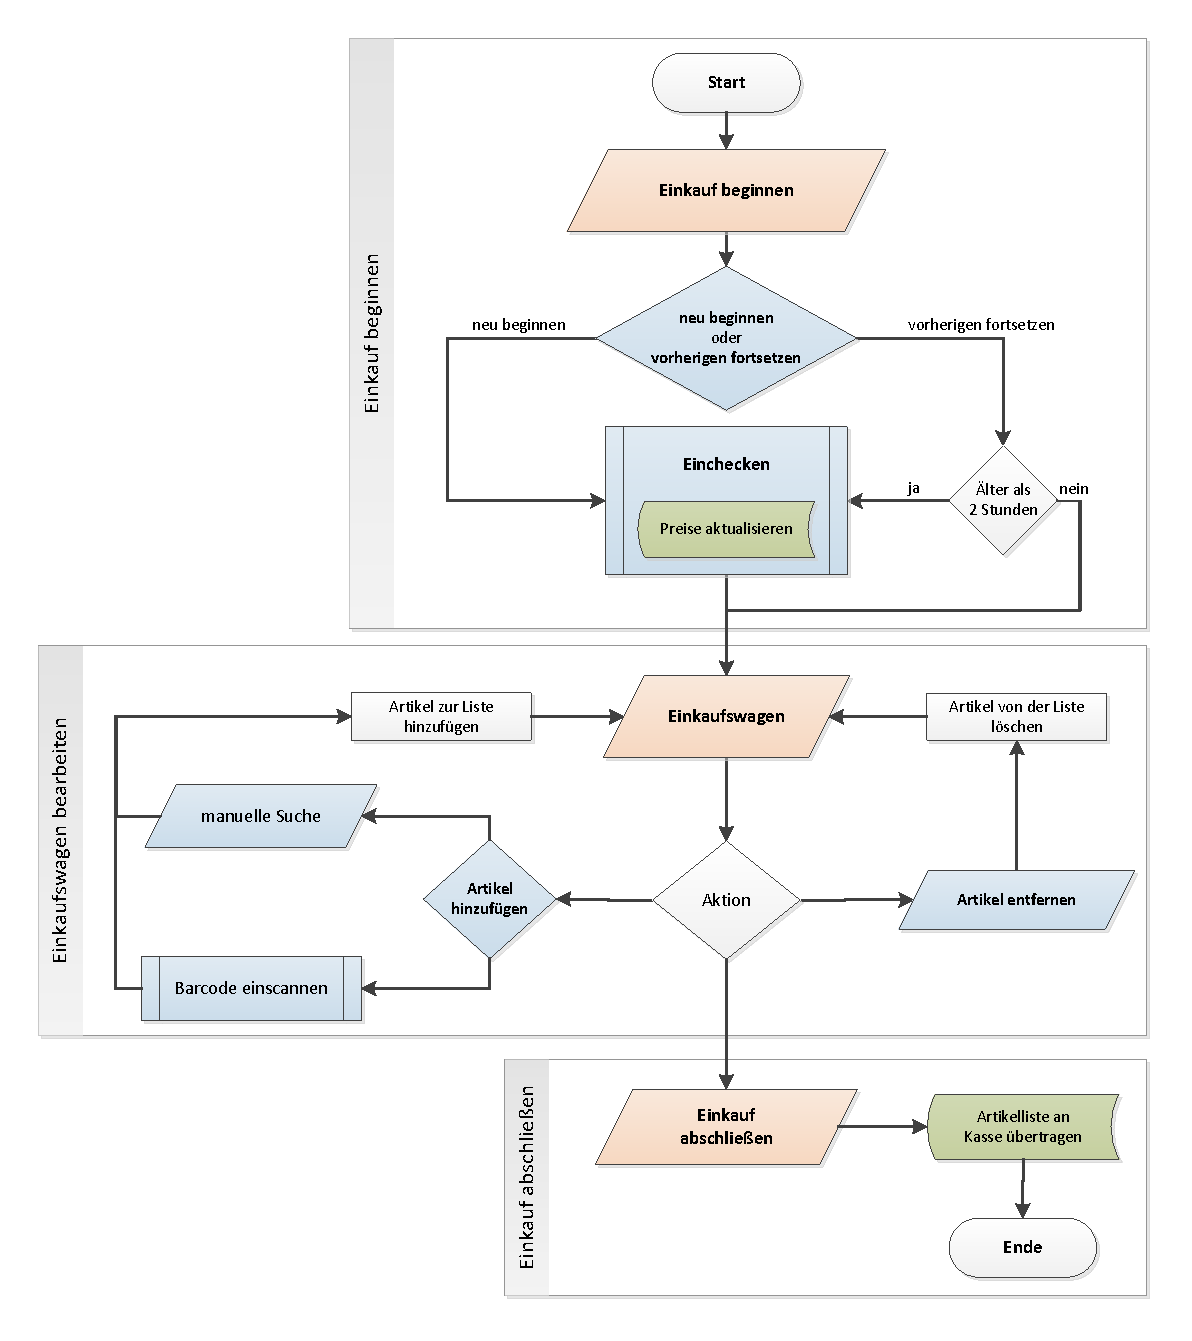
\includegraphics[width=\linewidth]{res/ablaufdiagramm_v2.pdf}
\caption{Der Einkaufsprozess mithilfe einer Self-Scanning Anwendung als Flussdiagramm}\label{abb:gesamtkonzept}
\end{figure}

Der Einkaufsprozess gliedert sich in drei Teilprozesse, die in der Grafik durch ein Rechteck gruppiert werden: Einkauf beginnen, Einkaufswagen bearbeiten und Einkauf abschließen. Benutzerdialoge sind gekennzeichnet durch ein rot hinterlegtes Trapez. Ein blaues Element beschreibt eine Benutzeraktion, ein graues steht dagegen für eine Funktion der Anwendung. Letztlich sind noch die zwei Schnittstellen (grün) zu erwähnen: Preise aktualisieren und Artikelliste an Kasse übertragen.

Die drei Teilprozesse Einkauf beginnen, Einkaufswagen bearbeiten und Einkauf abschließen werden in den folgenden Unterkapiteln näher erläutert.

\subsection{Einzelne Teilprozesse im Detail}\label{konzept:teilprozesse}

\subsubsection*{Einkauf beginnen}
Im ersten Schritt soll der Kunde zunächst entscheiden, ob er einen neuen Einkauf beginnen oder einen vorherigen fortsetzen möchte. Da sich einzelne Artikelpreise von Filiale zu Filiale unterscheiden können, ist die Information über den aktuellen Standort des Kunden eine zentrale Voraussetzung für den Einkauf mit dem Smartphone. Hierfür wird vor jedem neuen Einkauf ein Zwischenschritt eingeführt, der im Folgenden „Einchecken“ genannt wird.

Beim Einchecken greift die Anwendung auf eine Schnittstelle der Filiale zu, um alle für den Einkauf notwendigen Informationen auf das Smartphone zu übertragen. Die konkreten Anforderungen, die sich an diese Schnittstelle ergeben, werden in \vref{anforderung:einchecken} beschrieben.

%Zum Einchecken scannt der Kunde einen QR-Code im Eingangsbereich der Filiale, in dem . Hierbei lassen sich zusätzliche Informationen an das Smartphone übertragen, die für den Einkauf notwendig sind (bspw. Preisveränderungen, die erst kurz vor dem Einkauf entstanden sind). Eine detaillierte Beschreibung dieser Schnittstelle folgt im [Kapitel: Schnittstellendefinition – Smartphone->Kasse].

Für den Fall, dass der Nutzer während eines Einkaufs unterbrochen wird (z.\,B. durch einen eingehenden Anruf), hat er die Möglichkeit, einen bereits angefangenen Einkauf fortzuführen. Daran knüpft sich die Bedingung, dass das Erstellungsdatum des Einkaufs nicht länger als 2 Stunden in der Vergangenheit liegt. Ansonsten ist eine Aktualität der Preise nicht mehr gewährleistet. Der Nutzer müsste in diesem Fall erneut einchecken.

\subsubsection*{Einkaufswagen bearbeiten}
Nachdem ein neuer Einkauf eröffnet bzw. ein unterbrochener fortgesetzt wurde, befindet sich der Kunde im „Einkaufswagen“-Dialog. Hier werden alle bisher erfassten Artikel in einer Liste aufgeführt. Neue Artikel können der Liste hinzugefügt oder bestehende von der Liste entfernt werden.

Das Hinzufügen von Artikeln kann auf zwei Weisen erfolgen: entweder per Einscannen des Barcodes auf der Artikelverpackung oder per manueller Suche, für den Fall, dass Verpackung oder Barcode nicht vorhanden sind. Die Suche soll dann anhand Artikelbezeichnung oder -nummer ermöglicht werden.

\subsubsection*{Einkauf abschließen}
Sobald sich alle Artikel im Einkaufswagen befinden, kann der Kunde seinen Einkauf an einer der herkömmlichen Kassen bezahlen. Hier greift die Anwendung auf eine zweite Schnittstelle zu, um die vom Kunden eingescannten Artikel an das Kassensystem zu übertragen. Die konkreten Anforderungen, die sich an diese Schnittstelle ergeben, werden in \vref{anforderung:kasse} beschrieben.

\section{Anforderungsermittlung}\label{anforderungen}

\subsection{Fachliche Anforderungen}
Anhand des in der ersten Projektarbeit erarbeiteten und im vorherigen Kapitel zusammengefassten Lösungskonzepts sollen nun fachliche und technische Anforderungen definiert und nummeriert werden.

\begin{seToplist}{xxxxx}
	\item[F01] Der Kunde soll seinen Einkauf mithilfe einer mobilen Anwendung durchführen können. Der gesamte Prozess lässt sich in die drei folgenden Bestandteile gliedern, deren detaillierte Beschreibung in \ref{konzept:teilprozesse} zu finden ist:
	\begin{seToplist}{xxx}
		\item[a]\textit{Einkauf beginnen}
		\item[b]\textit{Einkaufswagen bearbeiten}
		\item[c]\textit{Einkauf abschließen}
	\end{seToplist}
	\item[F02] An die Stammdaten, d.\,h. die Artikel- und Preisinformationen, die der Anwendung zur Verfügung stehen, ergeben sich folgenden Unteranforderungen:
	\begin{seToplist}{xxx}
		\item[a]\textit{Verfügbarkeit der Daten}\\
		Während des Einkaufs soll weder eine Verbindung zum Internet noch eine Verbindung zum Kassensystem oder dem Filialnetzwerk erforderlich sein.
		\item[b]\textit{Vollständigkeit der Artikel}\\
		Jeder Artikel der in der Filiale erworben werden kann, soll mithilfe des Smartphones erfasst werden können. Dazu gehören ausdrücklich auch unverpackte bzw. lose Waren (z.\,B. aus der O\&G-Abteilung oder dem Backautomaten). Darüber hinaus sollen auch sog. Gewichtsartikel (Artikel deren Preis abhängig vom Gewicht ist) sowie Pfandbons dem virtuellen Einkaufswagen hinzugefügt werden können.
		\item[c]\textit{Abweichungen einzelner Filialen}\\
		Auch „lokale Preisveränderungen“ sollen berücksichtigt werden. Darunter werden Preisabweichungen verstanden, die lediglich innerhalb einer Filiale für einen begrenzten Zeitraum gültig sind (z.\,B. beim Abverkauf von O\&G kurz vor Feierabend), .
		\item[d]\textit{Aktualität der Preise}\\
		Die Preisinformationen sollen stets mit den aktuell gültigen Preisen der Filiale übereinstimmen. Toleriert werden lediglich Preisänderungen, die nach dem Einchecken vorgenommen werden.
	\end{seToplist}
	\item[F03]Die im Dialog Einkaufswagen anzuzeigenden Informationen werden in der \ref{tab:einkaufswagen} in der Übersicht dargestellt:
	
	\begin{table}[H]
	  \begin{center}\small\renewcommand{\arraystretch}{1.4}\sffamily % kleinere, serifenlose Schrift & größere Zeilen
	  \begin{tabulary}{\textwidth}{lllll}
	  	\multicolumn{5}{c}{Aktuelle Filiale des Kunden}\\ \hline
	    \multirow{2}{*}{Menge} & \multicolumn{3}{l}{Artikelbezeichnung} & \multirow{2}{*}{Gesamtpreis}\\ \cline{2-4}
	    & EAN & Einzelpreis & MwSt.-Satz & \\ \hline
	    \multicolumn{5}{c}{\multirow{2}{*}{\textit{weitere Artikelpositionen}}}\\
	    \multicolumn{5}{c}{} \\\cline{1-4}\hhline{~~~~=}
	    \multicolumn{4}{l}{Zwischensumme der Steuersätze} & Summe \\
	   \end{tabulary}      
	 \caption{Tabellarische Darstellung der Inhalte im Dialog: Einkaufswagen}
	 \label{tab:einkaufswagen}
	 \end{center} 
	\end{table}
	
	\item[F04] In einigen Fällen führt das Erfassen von Artikeln zu Ausnahmen. Diese werden im Folgenden erläutert:
	\begin{seToplist}{xxx}
		\item[a]\textit{Preisanzeige von Gewichtsartikeln}\\
		In der Filiale befinden sich keine für den Kunden zugänglichen Waagen. Der Preis eines Gewichtsartikels soll deshalb lediglich in Bezug auf eine Grundeinheit angezeigt werden (z.\,B. 1,99 \euro/kg). Zusätzlich soll ein Hinweis erscheinen, dass der Artikel an der Kasse noch gewogen werden muss.
		\item[b]\textit{Altersbeschränkung bei Artikeln}\\
		Beim Erfassen von Artikeln mit Altersbeschränkung (z.\,B. Spirituosen) soll ein Hinweis erscheinen, dass die Volljährigkeit des Kunden an der Kasse zunächst kontrolliert werden muss.
		\item[c]\textit{Abweichung vom tatsächlich zu zahlenden Betrag}\\
		Die Bonsumme, die der Kunde auf dem Smartphone angezeigt bekommt, könnte von der Summe abweichen, die er tatsächlich zu zahlen hat (z.\,B. bei einer Preisveränderung während des Einkaufs). Dies sollte vom Kassensystem überprüft und den Kunden ggf. darauf hinweisen.	
	\end{seToplist}
\end{seToplist}

\subsection{Technische Anforderungen}\label{anforderungen-technisch}

\label{anforderung:einchecken}
\begin{seToplist}{xxxxx}
	\item[T01]Beim Einchecken greift die Anwendung auf eine Schnittstelle zu, mit dessen Hilfe die folgenden Informationen abgerufen werden sollen:
	\begin{seToplist}{xxx}
		\item[a]\textit{Ermittlung des Standorts}\\
		Aufgrund der fachlichen Anforderung \textit{F02c Abweichung einzelner Filialen} muss vor jedem Einkauf die aktuelle Filiale des Kunden ermittelt werden. Die entsprechenden Standortdaten sollen beim Einchecken an das Smartphone übermittelt werden.
		\item[b]\textit{Aktualisierung der lokalen Preise}\\
		Darüber hinaus fordert die Anforderung \textit{F02d Aktualität der Preise}, dass die in der Anwendung anzuzeigenden Preise mit denen der Filiale stets übereinstimmen sollen. Um dies sicherzustellen sollen auch aktuelle Preisveränderungen der Filiale von der Schnittstelle bereitgestellt werden.
	\end{seToplist}
	\item[T02]\label{anforderung:kasse}Bei der Bezahlung erfolgt ein weiterer Informationsaustausch mit dem Kassensystem: die erfassten Artikel müssen an die Kasse übertragen werden, um den Einkauf anschließend bezahlen zu können. Von der Kasse werden folgende Informationen benötigt:
	\begin{seToplist}{xxx}
		\item[a]\textit{Standortdaten}\\
		Zur erneuten Prüfung, ob der Standort des Kunden mit der tatsächlichen Filiale übereinstimmt, sollen die beim Einchecken empfangenen Standortdaten auch der Kasse bereitgestellt werden.
		\item[b]\textit{Details zu Artikelpositionen}\\
		Für jeden Artikel im Einkaufswagen soll lediglich Artikelnummer und die zugehörige Menge zur Kasse übertragen werden.
		\item[c]\textit{Gesamtsumme des Einkaufswagens}\\
		Um zu prüfen, ob die in der Anwendung berechnete Summe mit dem tatsächlich zu zahlenden Betrag übereinstimmt (siehe \textit{F04c Abweichung vom tatsächlich zu zahlenden Betrag}), soll auch die berechnete Summe an die Kasse übertragen werden.
	\end{seToplist}
	\item[T03]An die Vorgehensweise zur Entwicklung mobiler Applikationen ergeben sich folgende technische Anforderungen:
	\begin{seToplist}{xxx}
		\item[a]\textit{Kamerazugriff} zum Erfassen von Barcodes
		\item[b]\textit{Datenspeicher} zur permanenten Ablage von Artikel- und Preisdaten.
		\item[c]\textit{Zugriff auf Internetverbindung}, zur Aktualisierung der Daten.
		\item[d]\textit{Kurzfristige Entwicklungsergebnisse}, aufgrund der zeitlichen Begrenzung des Projekts, sowie des prototypischen Charakters. Das Hauptaugenmerk soll weniger auf Performance oder Usability liegen, sondern vielmehr auf einer kurzen Entwicklungszeit und raschem Erkenntnisgewinn (steile Lernkurve).
	\end{seToplist}
\end{seToplist}

\section{Kapitelzusammenfassung}
Dem Kunden soll die Möglichkeit geboten werden, alle Artikel bereits während des Einkaufs in einer Filiale mithilfe seines Smartphones zu erfassen und in einer Liste zu speichern. Das Erfassen wird durch das Einscannen eines Barcodes auf der Artikelverpackung oder alternativ durch manuelles Suchen in einer Artikeldatenbank ermöglicht. Die Liste aller eingescannten Artikel wird bei der Bezahlung an das Kassensystem übertragen, sodass der Einkauf an einer herkömmlichen Kasse bezahlt werden kann. Das Auflegen der Artikel aufs Kassenband, anschließende Einscannen und erneute Einpacken an der Kasse entfällt somit.


\chapter{Vorgehensweisen zur Entwicklung mobiler Anwendungen}

\section{Kapiteleinleitung}
Ausgehend von den in \ref{anforderungen} definierten Anforderungen, kann die mobile Applikation entworfen und implementiert werden. Zunächst sollen jedoch grundsätzliche Vorgehensweisen zur Entwicklung mobiler Applikationen vorgestellt und anhand der Anforderung an die Entwicklungsmethode (T03) bewertet werden, um abschließend eine für das Projekt passende Methode auszuwählen.

\section{Beschreibung der einzelnen Vorgehensweisen}

\subsection{Entwicklung einer nativen App}
Als native Apps werden eigenständige Anwendungen bezeichnet, die speziell für ein konkretes Betriebssystem implementiert werden und letztendlich nur auf diesem System installations- und lauffähig sind. Auf diese Weise können die Systemressourcen optimal ausgereizt und mithilfe entsprechender Grundkonzepte des jeweiligen Betriebssystems (Multithreading, Speicherzugriff, Grafikrendering) eine hohe Performance erzielt werden. Dieser Aspekt macht sich besonders bei komplexen Anwendungen bemerkbar. Darüber hinaus ermöglichen native Apps den Zugriff auf Gerätekomponenten, wie z.B. Kamera, GPS-Sensor oder NFC-Chip.\seFootcite{Vgl.}{S. 381f}{Galileo:HTML5}
 
Neben den eben genannten Vorteilen auf technischer Seite, gibt es noch einen weiteren, marketingtechnischen Aspekt: native Apps werden über den offiziellen App-Store des jeweiligen Herstellers vertrieben. Potenziellen Nutzer können die App in gewohnter Art und Weise finden, Bewertungen lesen und die App gegebenenfalls direkt auf dem Smartphone installieren. Nach der Installation befindet sich eine Verknüpfung auf dem Homescreen des Nutzers, sodass die App jederzeit zur Verfügung steht.

Dieser Aspekt gilt jedoch gleichzeitig auch als Nachteil zu erwähnen: vor der Veröffentlichung im App-Store von Apple zunächst ein aufwendiger Freigabeprozess durchlaufen werden. Die App kann jederzeit vom Store-Betreiber abgelehnt oder nachträglich aus dem Store entfernt werden. Außerdem ist für die offizielle Entwicklung einer nativen App im Falle von Apple eine kostenpflichtige Lizenz sowie ein Mac Voraussetzung.
%TODO Quelle angeben!

Hinzu kommt die aufwendige Einarbeitung für unerfahrene Entwickler. Selbst bei guter Kenntnis der zu implementierenden Sprache ist eine sorgfältige Einarbeitung in das jeweilige SDK unverzichtbar. \seFootcite{Vgl.}{S. 382}{Galileo:HTML5}

\vref*{tab:procon-nativ} zeigt die eben genannten Vor- und Nachteile in der Übersicht.

\begin{table}[H]
  \begin{center}\small\renewcommand{\arraystretch}{1.4}\sffamily % kleinere, serifenlose Schrift & größere Zeilen
    \begin{tabulary}{\textwidth}{>{\raggedleft}m{61mm} *{2}{>{\ttfamily}m{5mm}} m{61mm}}
    \multicolumn{2}{r}{\textbf{Vorteile}}	&	\multicolumn{2}{l}{\textbf{Nachteile}}\\ \hline
    
    Hohe Performance, auch bei komplexen Anwendungen & (+) &
    (-) & Aufwendiger Freigabeprozess\\
    
    Einfacher und umfangreicher Zugriff auf Gerätekomponenten & (+) &
    (-) & Ggf. kostenpflichtige Entwicklerlizenzen erforderlich\\
    
    Effiziente Vermarktung über den App-Store & (+) & (-) & Äußerst zeitintensive Einarbeitung notwendig\\
    
    Schneller Zugriff durch Verknüpfung auf dem Homescreen & (+) & & \\

    \end{tabulary}        
    
    \caption{Vor- und Nachteile bei der nativen App-Entwicklung}
    \label{tab:procon-nativ}
  \end{center}
\end{table}

\subsection{Entwicklung einer Web-App}
Eine Webanwendung wird im Gegensatz zur nativen App nicht eigenständig, sondern mithilfe eines Browsers auf dem Zielsystem ausgeführt, eine Installation ist nicht notwendig. Sie kann direkt durch manuelles Eingeben der URL oder Aufrufen eines Lesezeichens geöffnet werden. Im Regelfall wird keine Verknüpfung auf dem Homescreen erstellt. Eine Webanwendung unterscheidet sich nur geringfügig von einer herkömmlichen Webseite. Die größten Unterschiede liegen in der für mobile Geräte optimierten Bedienoberfläche und dem reduzierten Funktions- und/oder Informationsumfang.\seFootcite{Vgl.}{}{GIA:ProCon}

Die Möglichkeiten einer Web-App werden durch den jeweiligen Browser begrenzt, in dem die App ausgeführt wird. Funktionen, die innerhalb des Browsers nicht zur Verfügung stehen, können von der App nicht verwendet werden. So gibt es beispielsweise keine Möglichkeit, den Nutzer einer Web-App per Push-Notification zu kontaktieren. 

Dank moderner Webtechnologien wie HTML5 stehen allerdings zahlreiche Möglichkeiten für den Zugriff auf Systemkomponenten zur Verfügung. Der Anwender muss diesen Zugriff leider jedes Mal explizit gewähren. Darüber hinaus ermöglicht der sog. DOM-Storage eine permanente lokale Datenspeicherung bis zu 5 bzw. 10MB – je nach verwendetem Browser. Die zusätzliche Integration zahlreich vorhandener JavaScript-Frameworks ermöglicht dem Entwickler auch komplexe Applikationen schnell und einfach zu entwickeln.

Eine Webanwendung muss lediglich einmal implementiert werden und ist dank der einheitlichen Webstandards auf allen Betriebssystemen lauffähig. Zur Veröffentlichung ist weder ein Freigabeprozess noch eine Lizenz notwendig. Es genügt ein Webserver auf dem die Anwendung läuft.

\vref*{tab:procon-webapp} zeigt die eben genannten Vor- und Nachteile in der Übersicht.

\begin{table}[H]
  \begin{center}\small\renewcommand{\arraystretch}{1.4}\sffamily % kleinere, serifenlose Schrift & größere Zeilen
    \begin{tabulary}{\textwidth}{>{\raggedleft}m{61mm} *{2}{>{\ttfamily}m{5mm}} m{61mm}}
    \multicolumn{2}{r}{\textbf{Vorteile}}	&	\multicolumn{2}{l}{\textbf{Nachteile}}\\ \hline
    
    Keine Installation notwendig & (+) &
    (-) & Aufwendiger Aufruf über den Browser, kein direkter Zugriff über Verknüpfung auf dem Homescreen\\
    
    Auf verschiedenen Betriebssystemen lauffähig & (+) & (-) & Limitierter Funktionsumfang, je nach verwendetem Browser\\
    
    Zugriff auf Gerätekomponenten dank HTML5 möglich & (+) & (-) & Zugriff auf Gerätekomponenten muss jedes Mal gewährt werden\\
    
    Komplexe Anwendungen durch Verwendung zusätzlicher Frameworks möglich & (+) & &\\
    
    Kein Freigabeprozess oder Lizenz notwendig & (+) & &

    \end{tabulary}        
    
    \caption{Vor- und Nachteile bei der Entwicklung einer WebApp}
    \label{tab:procon-webapp}
  \end{center}
\end{table}

\subsection{Entwicklung einer hybriden App}\label{kapitel:procon-hybrid}
Hybride Apps vereinen die Vorteile beider Entwicklungsalternativen: sie werden zunächst als WebApp implementiert und anschließend in eine native App eingebettet. Die native App besitzt einen sog. InApp-Browser, in dem die ursprünglich entwickelte Webanwendung gerendert wird.

Auf diese Weise können mobile Anwendungen mithilfe der bekannten Webtechnologien entwickelt werden, sind auf verschiedenen Betriebssystemen lauffähig und bieten dank der umgebenden nativen App trotzdem den vollen Funktionsumfang (d.\,h. hybride Apps ermöglichen bspw. auch die Verwendung von Push-Notifications).

Für den Nutzer sind hybride Apps von nativen kaum zu unterscheiden, da sie wie gewohnt über den App-Store heruntergeladen, installiert und über eine Verknüpfung auf dem Homescreen aufgerufen werden. Lediglich in der Benutzeroberfläche lässt sich ein Unterschied erkennen, da für das Rendering nicht die nativen Bedienelemente, sondern lediglich HTML5 und CSS3 Komponenten verwendet werden.

\vref*{tab:procon-hybrid} zeigt die eben genannten Vor- und Nachteile in der Übersicht.

\begin{table}[H]
  \begin{center}\small\renewcommand{\arraystretch}{1.4}\sffamily % kleinere, serifenlose Schrift & größere Zeilen
    \begin{tabulary}{\textwidth}{>{\raggedleft}m{61mm} *{2}{>{\ttfamily}m{5mm}} m{61mm}}
    \multicolumn{2}{r}{\textbf{Vorteile}}	&	\multicolumn{2}{l}{\textbf{Nachteile}}\\ \hline
    
    Einfache Implementierung als Webanwendung & (+) &
    (-) & Keine nativen Bedienelemente\\
    
    Lauffähig auf verschiedenen Betriebssystemen & (+) & & \\
    
    Funktionsumfang einer nativen App & (+) & & \\
    
    Vermarktung, Installation und Aufruf wie bei einer nativen App & (+) & &\\

    \end{tabulary}        
    
    \caption{Vor- und Nachteile bei der hybriden App-Entwicklung}
    \label{tab:procon-hybrid}
  \end{center}
\end{table}

\section{Bewertung und Auswahl einer Vorgehensweise}
Der Vergleich der drei Herangehensweisen verdeutlichte, dass jede Entwicklungsmethode äußerst unterschiedliche Vor- und Nachteile mit sich bringt. Inwiefern die technischen Anforderungen an die Entwicklungsmethode aus \ref{anforderungen-technisch} erfüllt werden, soll \vref{tab:procon-auswertung} zeigen.

\begin{table}[H]
  \begin{center}\small\renewcommand{\arraystretch}{1.4}\sffamily % kleinere, serifenlose Schrift & größere Zeilen
    \begin{tabulary}{\textwidth}{cl*{3}{>{\ttfamily}c}}
    \textbf{ID} & \textbf{Bezeichnung} & \sffamily\textbf{nativ} & \sffamily\textbf{web} & \sffamily\textbf{hybrid}\\ \hline
    
    T03a & Kamerazugriff & (+) & (-) & (+) \\
    T03b & Datenspeicher & (+) & (-) & (+) \\
    T03c & Internetzugriff & (+) & (+) & (+) \\
    T03d & Entwicklungszeit & (-) & (+) & (+)

    \end{tabulary}        
    
    \caption{Erfüllung der an die Entwicklungsmethode gestellten Anforderungen}
    \label{tab:procon-auswertung}
  \end{center}
\end{table}

Aufgrund der Tatsache, dass der Zugriff auf Kamera und Datenspeicher bei Verwendung einer WebApp jedes Mal gewährt werden muss, wird diese Vorgehensweise nicht weiter betrachtet.

Die Implementierung als native App wäre aufgrund der hohen Menge an Artikel- und Preisdaten und der damit einhergehenden Rechenlast sicherlich die richtige Vorgehensweise. Im Rahmen dieses Projektes liegt der Fokus jedoch nicht auf Performance, sondern auf einer kurzen Entwicklungszeit. Vor diesem Hintergrund soll die Self-Scanning Anwendung als hybride App entworfen und implementiert werden.

\section{Kapitelzusammenfassung}
Die drei unterschiedlichen Vorgehensweisen zur App-Entwicklung wurden zunächst vorgestellt und deren Vor- und Nachteile herausgearbeitet. Die tabellarische Übersicht am Ende jedes Kapitels verdeutlichte die wesentlichen Punkte:
\begin{itemize}
	\item native Apps erzielen selbst bei komplexen Anwendungen eine hohe Performance, der nötige Entwicklungsaufwand ist jedoch für unerfahrene Entwickler besonders hoch.
	\item Webanwendung lassen sich dagegen mithilfe bekannter Webtechnologien entwickeln und ohne weitere Umstände veröffentlichen. Der vom Nutzer verwendete Browser limitiert den Funktionsumfang jedoch.
	\item hybride Apps vereinen die Vorteile beider Alternativen: äußerst einfache Entwicklung dank bekannter Webtechnologien und gleichzeitig den vollen Funktionsumfang dank der umgebenden nativen App.
\end{itemize} 

Die Entwicklung einer reinen Web-App wurde aufgrund des eingeschränkten Zugriffs auf Gerätekomponenten ausgeschlossen. Der entscheidende Vorteil einer hybriden App gegenüber einer nativen App liegt in der sehr viel kürzeren Entwicklungszeit, weshalb die Self-Scanning Anwendung im folgenden Kapitel als hybride Applikation entworfen werden soll.

\chapter{Entwurf der Self-Scanning App}
\section{Kapiteleinleitung}
Das in \vref{kap:konzept} erläuterte Konzept soll nun anhand der ermittelten Anforderungen als mobile Anwendung entworfen und implementiert werden.

Hierfür soll zunächst die grundlegende Struktur einer hybriden App und die daraus resultierende Architektur der Anwendung beschrieben werden. Anschließend werden einzelne Prozesse und Schnittstellen zu externen Systemen ausführlich erläutert.

\section{Die Architektur der Anwendung}
\subsection{Grundlegende Struktur einer PhoneGap-Anwendung}
PhoneGap ermöglicht dem Entwickler, webbasierte Anwendungen in eine native App zu packen. Gleichzeitig wird der Webanwendung eine Schnittstelle zur nativen App bereitgestellt, sodass die Anwendung im Inneren auf die nativen Geräte- und Systemkomponenten zugreifen kann.\seFootcite{Vgl.}{}{AB:Compare}
\vref{abb:phonegap} veranschaulicht diesen sog. Packaging-Prozess und den daraus resultierenden Aufbau einer PhoneGap-Anwendung.

\begin{figure}[H]
	\centering
	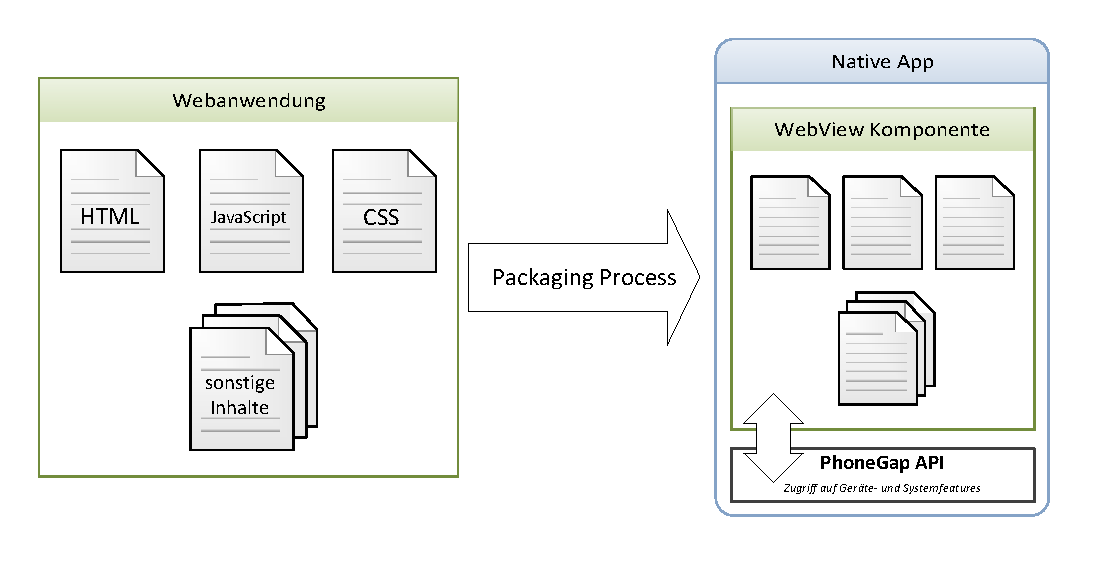
\includegraphics[width=.9\linewidth]{res/phonegap.pdf}
	\caption{Packaging-Prozess von PhoneGap und Aufbau einer hybriden App\protect\footnotemark}\label{abb:phonegap}
\end{figure}
\protect\footnotetext{in Anlehnung an \seCite{}{S. 6}{PG:Wargo}}

Die konkrete Gestaltung von Datenhaltung, Programmlogik und Benutzeroberfläche, wird von PhoneGap jedoch nicht vorgegeben. Hierfür soll Sencha Touch zum Einsatz kommen -- ein JavaScript Framework, welches einerseits eine möglichst nativ wirkende Benutzeroberfläche schafft und andererseits ein Grundgerüst für die Architektur der Webanwendung schafft. Ein wichtiger Bestandteil dieses Frameworks ist das MVC-Konzept, welches im folgenden Unterkapitel näher vorgestellt werden soll.

\subsection{Prinzipien und Bestandteile des MVC-Konzepts}
Das MVC-Konzept entspringt der Idee des sog. Beobachter-Musters. Diesem Muster zufolge wird zwischen Objekten unterschieden, welche die Rolle eines Beobachters einnehmen und solchen, die beobachtet werden. Beobachtete Objekte kennen ihre Beobachter, sodass letztere benachrichtigt werden können, sobald sich der Zustand eines beobachteten Objekts ändert. Die Beobachter-Objekte können außerdem den aktuellen Zustand der beobachteten Objekte jederzeit erfragen.\seFootcite{Vgl.}{S. 512f}{OO:Handbuch}

Darüber hinaus wird die strikte Trennung von Datenhaltung, Darstellung und Steuerung verfolgt. Diese drei Bestandteile werden als Model, View und Controller bezeichnet. Durch diese Aufteilung wird das System sehr leicht skalierbar und bleibt dennoch flexibel. Es können beispielsweise weitere Views unabhängig von Model oder Controller hinzugefügt, bestehende Views ausgetauscht oder entfernt werden.

Die drei zentralen Begriffe Model, View und Controller sollen im Folgenden etwas näher erläutert werden, um daraufhin den Bezug zum Beobachter-Muster herzustellen.

\paragraph{Das Model} enthält fachlich strukturierte Informationen\seFootcite{Vgl.}{S. 247}{EffSoftArch} und verwaltet in seinen Instanzen jeweils einen konkreten Zustand. Außerdem kann eine Model-Instanz Informationen zu seinem Zustand liefern oder diesen bei Bedarf ändern.\seFootcite{Vgl.}{S. 516}{OO:Handbuch}

\paragraph{Der View} hingegen ist ausschließlich für die Darstellung (Ausgabe) der Daten zuständig. Der entsprechende Input hierfür wird von den Models geliefert. Außerdem hat ein View die Zusatzaufgabe Benutzereingaben entgegenzunehmen und diese an den Controller weiterzuleiten. %TODO Quelle?!

\paragraph{Der Controller} hatte ursprünglich die Aufgabe, Benutzerinteraktionen zu verarbeiten (bspw. um einen Mausklick einem konkreten Button zuzuordnen). Diese Aufgaben werden mittlerweile jedoch von Modulen übernommen, die in Betriebssystem, Browser oder Basisbibliotheken integriert sind.\seFootcite{Vgl.}{S. 515}{OO:Handbuch}\\
Ein Controller im heutigen Sinne ist für die Ablaufsteuerung einer Anwendung und die Ausführung entsprechender Operationen zuständig. Typisches Beispiel hierfür ist die Änderung der im Model enthaltenen Daten, nachdem der Benutzer ein Eingabeformular ausgefüllt und abgeschickt hat.

Das Prinzip des oben erwähnten Beobachter-Musters findet im Rahmen von MVC nun folgendermaßen Anwendung: 
\begin{itemize}
	\item[a)] \textbf{View beobachtet Model}\\
	Jeder View kann sich in die Beobachterliste eines Models eintragen. So kann das Model alle beobachtenden Views bei Aktualisierung der Daten benachrichtigen. Die Views wiederum aktualisieren dann bei Bedarf ihre Darstellung.
	\item[b)] \textbf{Controller beobachtet Views}\\
	Ein Controller kann Views beobachten, um im Falle von Benutzereingaben benachrichtigt zu werden. Der Controller holt sich die Eingaben bei Bedarf und leitet weitere Schritte ein.
\end{itemize}

\subsection{Sencha Touch als formgebendes Framework}
\subsubsection*{Grundlagen zu Sencha Touch}
Bei Sencha Touch handelt es sich um ein HTML5-Framework zur Entwicklung von Webanwendungen, die sich besonders zur Darstellung und Bedienung auf mobilen Geräten eignen.\seFootcite{Vgl.}{}{ST:Guide} Mithilfe von Sencha Cmd, einem zusätzlichen Tool des Frameworks, lässt sich durch den Befehl \texttt{sencha generate app HelloWorld HelloWorld} eine initiale Ordner- und Dateistruktur erzeugen, die in \vref{abb:filestructure} dargestellt ist.\seFootcite{Vgl.}{}{STCmd}

\begin{figure}[H]
	\centering
	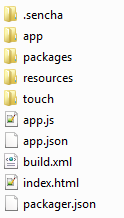
\includegraphics[scale=1]{res/filestructure.png}
	\caption{Dateistruktur einer initial erzeugten Sencha Touch Anwendung\protect\footnotemark}\label{abb:filestructure}
\end{figure}

\protect\footnotetext{eigene Darstellung}

Bei Ausführung der nativen Anwendung wird die \texttt{index.html} in den WebView (siehe \vref{abb:phonegap}) des mobilen Geräts geladen und angezeigt. Innerhalb der \texttt{index.html} werden nun weitere Bestandteile der Webanwendung eingebunden -- bspw. interne Bibliotheken des Frameworks (Ordner: \texttt{touch}), CSS-Dateien zur Gestaltung der Benutzeroberfläche (Ordner: \texttt{resources}), Konfigurationsdateien (Ordner: \texttt{.sencha}) und letztlich auch die \texttt{app.js}, in der die eigentliche Anwendung erzeugt und gestartet wird.

Das \vref{lst:helloworld} zeigt den Inhalt einer \texttt{app.js}-Datei, wodurch die App in \vref{abb:helloworld} erzeugt wird.

\begin{programm}[H]
	\begin{lstlisting}
Ext.application({
    name: 'HelloWorld',

    launch: function() {
        Ext.create('Ext.Container', {
            fullscreen: true,
            html: '<p>Hello, World!</p>'
        });
    }
});
	\end{lstlisting}
	\captionof{programm}{Die Datei \texttt{app.js} zur Erzeugung einer HelloWorld-App\label{lst:helloworld}}
\end{programm}

Darüber hinaus lassen sich vorgefertigte Model-, View- oder Controller-Klassen erzeugen und in die vorhandene Ordnerstruktur eingliedern. Über den Befehl\linebreak \lstinline|sencha generate controller -n einController| wird beispielsweise die Datei\linebreak \texttt{app/controller/einController.js} erstellt, mit dem Inhalt der in \vref{lst:helloworld-controller} zu sehen ist.

\begin{programm}[H]
	\begin{lstlisting}
Ext.define('HelloWorld.controller.einController', {
    extend: 'Ext.app.Controller',
    
    config: {
        refs: {
            
        },
        control: {
            
        }
    },
    
    //called when the Application is launched, remove if not needed
    launch: function(app) {
        
    }
});
	\end{lstlisting}
	\captionof{programm}{Das Grundgerüst einer Controller-Klasse\label{lst:helloworld-controller}}
\end{programm}

Die \texttt{launch()}-Funktion wird beim Start der Anwendung aufgerufen. Mithilfe der Eigenschaften \texttt{refs} und \texttt{control} lassen sich zu beobachtende Objekte und zugehörige eventHandler-Funktionen definieren.

\subsubsection*{Ergänzung zum MVC-Konzept}
Sencha Touch bietet neben den drei Standardkomponenten des MVC-Konzepts diverse zusätzliche Bausteine an. Im Folgenden sollen lediglich die für das Projekt relevanten Bestandteile von Sencha Touch beschrieben werden, um anschließend die Funktionsweise des Frameworks näher zu erläutern.

\paragraph{Der Store}\label{sencha-touch:stores} beinhaltet Model-Instanzen eines bestimmten Typs. Er stellt Funktionen bereit, um die Menge seiner Model-Objekte zu sortieren, zu gruppieren oder zu filtern. Außerdem können einzelne Model-Instanzen hinzugefügt, verändert oder entfernt werden.

\paragraph{Proxies }werden von Stores benutzt, um die Daten eines Models aus dem Speicher zu laden bzw. diese wieder in den Speicher zu schreiben. Bei dem Speichermedium muss es sich allerdings nicht immer um die lokale Festplatte handeln. Auch die Verbindung zu einer externen Datenbank oder einem Webservice wären denkbare Möglichkeiten.

\paragraph{Model-Assoziationen}
Zusätzlich zu den bekannten Eigenschaften eines Models bietet Sencha Touch die Möglichkeit, einzelne Model-Typen miteinander in Beziehung zu versetzen. Dabei werden die drei Beziehungstypen „belongsTo“, „hasOne“ und „hasMany“ unterschieden.\seFootcite{Vgl.}{Ext.data.association.Association}{ST:API} Anhand eines Beispiels lassen sich die Beziehung wie folgt erklären
\begin{itemize}
	\item[a)] belongsTo: jedes Auto gehört zu einem Besitzer
	\item[b)] hasMany: ein Besitzer kann mehrere Autos besitzen
	\item[c)] hasOne: jedes Auto hat genau einen Motor
\end{itemize}
Eine Model-Instanz kennt seine in Beziehung stehenden Model-Instanzen. Sencha Touch stellt auf Basis dieser Tatsache zusätzliche Funktionen bereit, um Model-Assoziationen zu traversieren. Im Falle des obigen Beispiels lässt sich also mithilfe einer Besitzer-Instanz (aufgrund der hasMany-Beziehung) ein Store erzeugen, der alle Autos dieses Besitzers enthält.

%Die \vref{abb:sencha-komponenten} verdeutlicht das Zusammenspiel der oben erläuterten Komponenten.

%\begin{figure}[H]
%	\centering
%	\includegraphics[width=\textwidth]{}
%	\caption{Zusammenspiel einzelner Sencha Touch Komponenten\protect\footnotemark}\label{abb:sencha-komponenten}
%\end{figure}

%\footnotetext{in Anlehnung an \seCite{}{}{ST:Guide}}

\subsection{Der Bezug zur Self-Scanning App}
\subsubsection*{Die drei Views der Anwendung}
Aus \vref{abb:gesamtkonzept} lassen sich die folgenden drei Benutzerdialoge erkennen: Einkauf beginnen, Einkaufswagen bearbeiten und Einkauf abschließen. Diese drei Dialoge entsprechen jeweils einem separaten View. Zusätzlich ist ein weiterer View für die manuelle Suche von Artikeln notwendig. Die folgende Abbildung veranschaulicht die zu erstellenden View-Klassen:

\begin{figure}[H]
	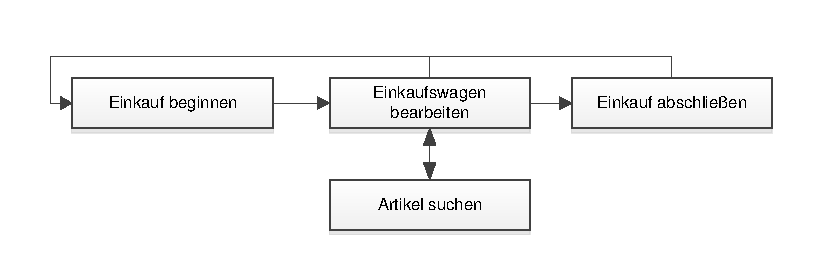
\includegraphics[width=\linewidth]{res/entwurf-views.pdf}
	\caption{Zu erstellende View-Klassen und deren Abfolge\protect\footnotemark}
\end{figure}

\protect\footnotetext{eigene Darstellung}

\subsubsection*{Models und die zugehörigen Assoziationen}
Anhand der fachlichen Anforderungen in \ref{anforderungen} und des prinzipiellen Ablaufs in \ref{prinzipieller-ablauf} wurden die in \ref{abb:models} dargestellten Model-Klassen identifiziert.

\begin{figure}[H]
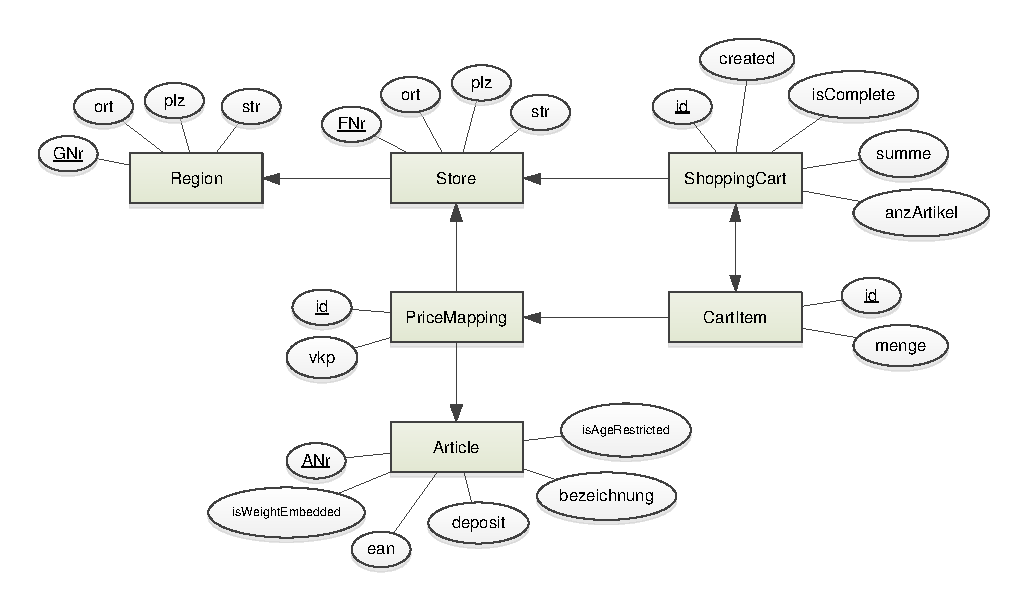
\includegraphics[width=\linewidth]{res/entwurf-models.pdf}
\caption{Zu implementierende Model-Typen und zugehörige Assoziationen}\label{abb:models}
\end{figure}

Die \texttt{Region}- und \texttt{Store}-Models repräsentieren Gesellschaften und Filialen, wobei jede Filiale zu genau einer Gesellschaft gehört. Folgende Vereinbarungen wurden (aus Gründen die gleich genannt werden) für die Eigenschaften von Gesellschaft und Filiale getroffen:
\begin{itemize}
	\item[a)] Die \texttt{Region} mit \texttt{GNr = 0} steht stellvertretend für alle Gesellschaften des Landes.
	\item[b)] Der \texttt{Store} mit \texttt{FNr = 0} steht stellvertretend für alle Filialen der \textit{jeweils zugehörigen} Gesellschaft.
	\item[c)] Ein \texttt{Store} mit \texttt{FNr = 0}, der zur \texttt{Region} mit \texttt{GNr = 0} gehört, steht stellvertretend für alle Filialen \textit{des Landes}.
\end{itemize}

Ein Artikel wird durch eine Model-Instanz vom Typ \texttt{Article} erstellt. Der Preis eines Artikels ist abhängig von der Filiale, in der sich der Kunde befindet. Hierfür wurde ein \texttt{PriceMapping}-Model eingeführt, das zu genau einer Filiale und zu genau einem Artikel gehört.

Durch die oben genannten Vereinbarungen lassen sich Preise auf unterschiedlichen Levels definieren:
\begin{itemize}
	\item[a)] Ein \texttt{PriceMapping}, das zu einem \texttt{Store} mit \texttt{FNr = 0} und \texttt{GNr = 0} gehört, ist ein \textbf{Landespreis}. D.\,h. er ist in allen Filialen des Landes gültig.
	\item[b)] Ein \texttt{PriceMapping}, das zu einem \texttt{Store} mit \texttt{FNr = 0} und \texttt{GNr $\neq$ 0} gehört, ist ein \textbf{Gesellschaftspreis}. D.\,h. er ist in allen Filialen dieser Gesellschaft gültig.
	\item[b)] Ein \texttt{PriceMapping}, das zu einem \texttt{Store} mit \texttt{FNr $\neq$ 0} und \texttt{GNr $\neq$ 0} gehört, ist ein \textbf{Filialpreis}. D.\,h. er ist ausschließlich in dieser Filiale gültig.
\end{itemize}

Der Preis für einen bestimmten Artikel wird in folgender Reihenfolge überschrieben und kann in umgekehrter Reihenfolge ermittelt werden:
\begin{center}
	\textbf{Landespreis > Gesellschaftspreis > Filialpreis}
\end{center}

Letztlich bleibt noch das \texttt{ShoppingCart}-Model, das alle Artikel enthält, die im Einkaufswagen liegen (\texttt{CartItems}). Jeder Einkaufswagen gehört zu genau einer Filiale. Jedes \texttt{CartItem} wiederum zu genau einem \texttt{PriceMapping}.

\subsubsection*{Stores und Proxies}
Zu jedem Model wird ein Store angelegt, der die von Sencha Touch bereitgestellten Standardfunktionen (siehe \vref{sencha-touch:stores}) anbietet.

Außerdem besitzt jedes Model einen eigenen Proxy, um die Daten in einer lokalen Datenbank abzuspeichern. Die Models \texttt{Region}, \texttt{Store}, \texttt{PriceMapping} und \texttt{Article} besitzen zusätzlich einen sog. „RemoteProxy“, der sich mit einer zentralen Datenbank im Internet verbindet und von dort aktuelle Informationen beziehen kann.

\subsubsection*{Der Controller}
Die Anwendung soll lediglich einen einzigen Controller enthalten, der alle drei Views gleichzeitig beobachtet und auf entsprechende Ereignisse reagiert. Hierdurch wird %TODO "warum hat nicht jeder View seinen eigenen Controller!?"

\begin{figure}[H]
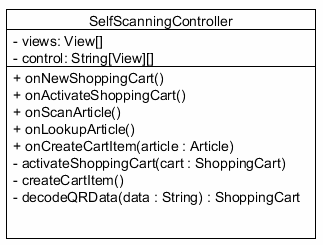
\includegraphics[scale=1]{res/controller.png}
\caption{Der zentrale Controller der Anwendung}
\end{figure}

\section{Der Entwurf einzelner Teilprozesse}
\subsection{Einkauf eröffnen}
\vref*{seq:einkauf-eroeffnen} zeigt den Prozess „Einkauf eröffnen“. Dieser wird angestoßen, wenn sich ein Nutzer im „Einkauf auswählen“-Dialog dafür entscheidet, einen neuen Einkauf zu beginnen. Hierfür ruft der Controller zunächst den Scanner auf, um den QR-Code im Eingangsbereich für den Check-In Prozess zu erfassen. Die darin enthaltenen Daten werden anschließend dekodiert und die entsprechenden Models (PriceMapping-Models) aktualisiert bzw. angelegt (ShoppingCart-Model). Das neu erstellte Model wird dann dem Einkaufswagen-View zugewiesen und angezeigt.

\begin{figure}[H]
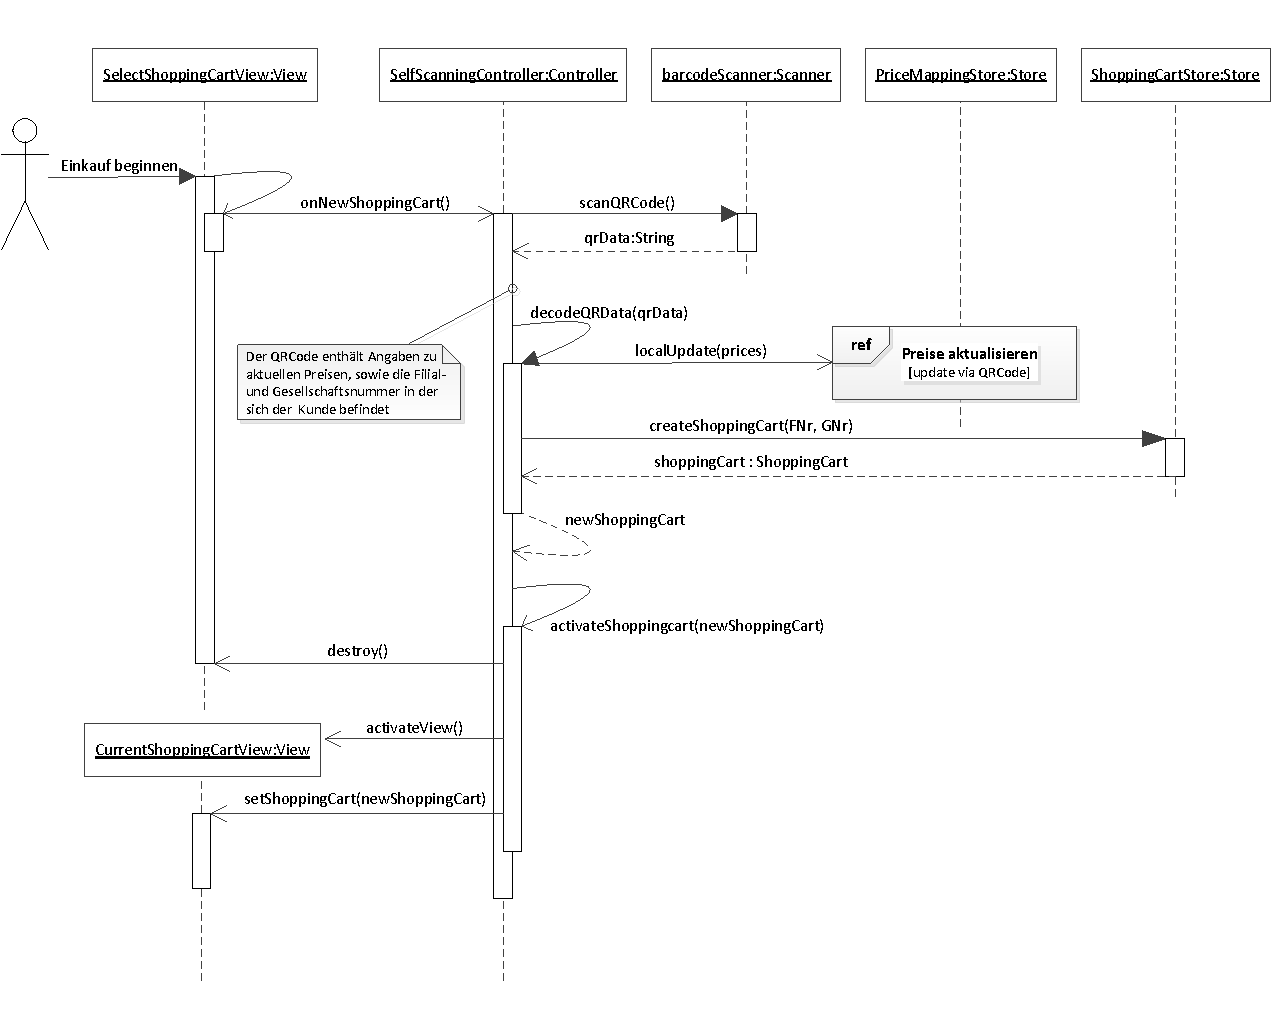
\includegraphics[width=\linewidth]{res/seq_einkauf-eroeffnen.pdf}
\caption{Der Prozess „Einkauf eröffnen“ als Sequenzdiagramm}\label{seq:einkauf-eroeffnen}
\end{figure}

\subsection{Artikel hinzufügen}
Um einen Artikel zu einem Einkaufswagen hinzuzufügen, bieten sich dem Nutzer zwei Möglichkeiten an: er scannt entweder den Barcode auf der Artikelverpackung oder sucht den passenden Artikel in einer Datenbank anhand Bezeichnung oder PLU-Nummer. Je nach Entscheidung werden die Methoden onScanArticle() bzw. onLookupArticle() ausgeführt, welche beide das passende Article-Model zurückliefern. Mit dessen Hilfe kann der Artikel dem aktuellen Einkaufswagen hinzugefügt und angezeigt werden.

\begin{figure}[H]
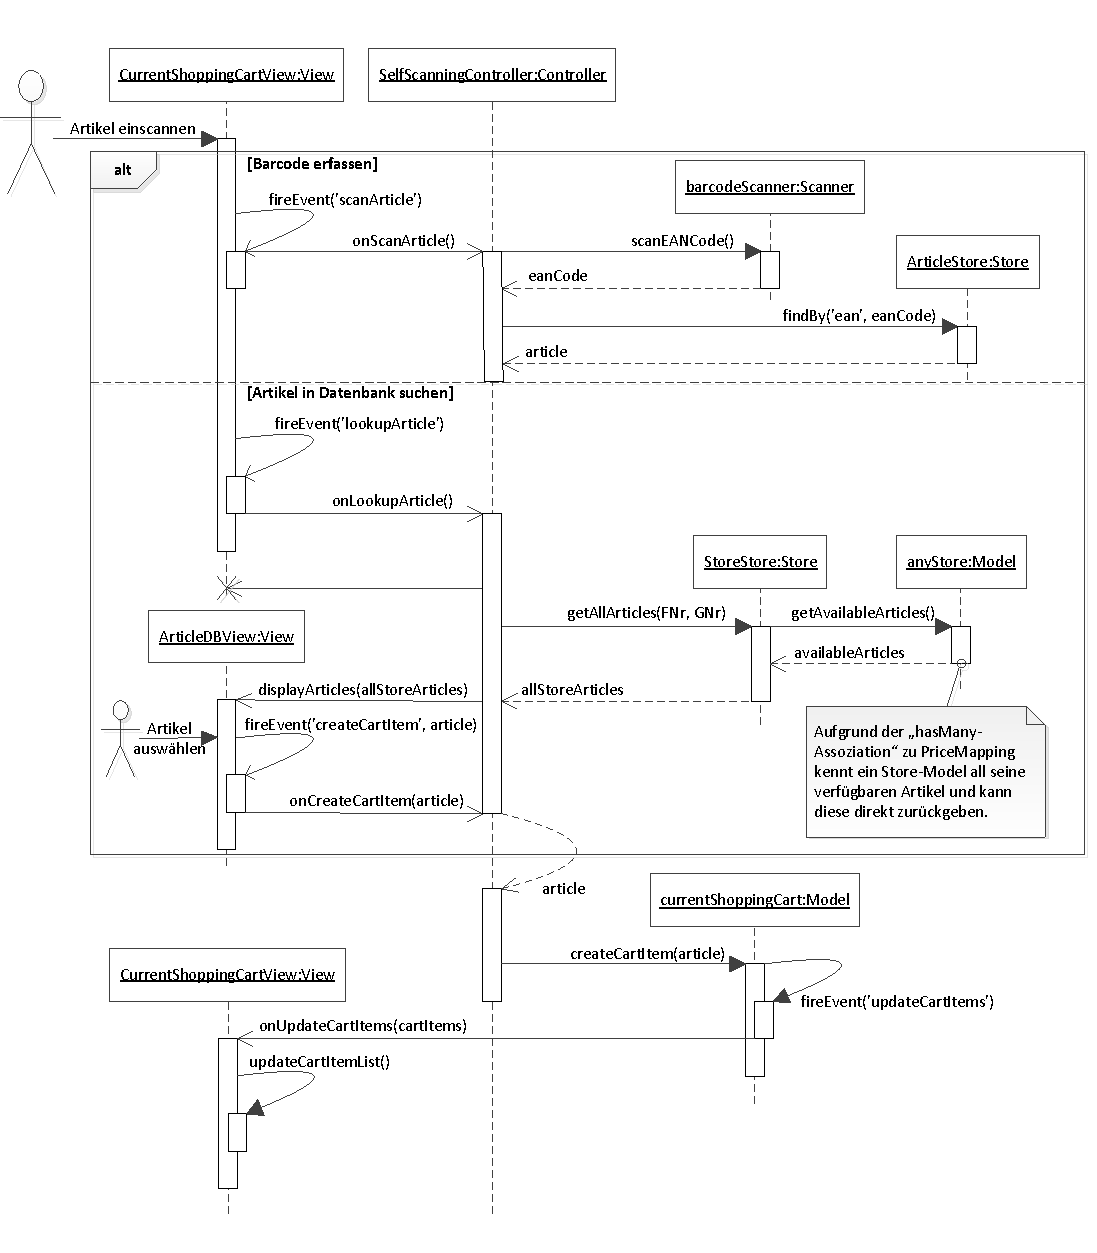
\includegraphics[width=\linewidth]{res/seq_artikel-hinzufuegen.pdf}
\caption{Der Prozess „Artikel hinzufügen“ als Sequenzdiagramm}
\end{figure}

\subsection{Preise aktualisieren}
Preise lassen sich entweder anhand des QR-Codes beim Check-In aktualisieren oder nach Anstoßen der remoteUpdate()-Funktion, um ein Update über das Internet durchzuführen. Letzteres erfolgt über den PriceMappingProxy, der von einer zentralen Datenbank seine Daten bezieht.

\begin{figure}[H]
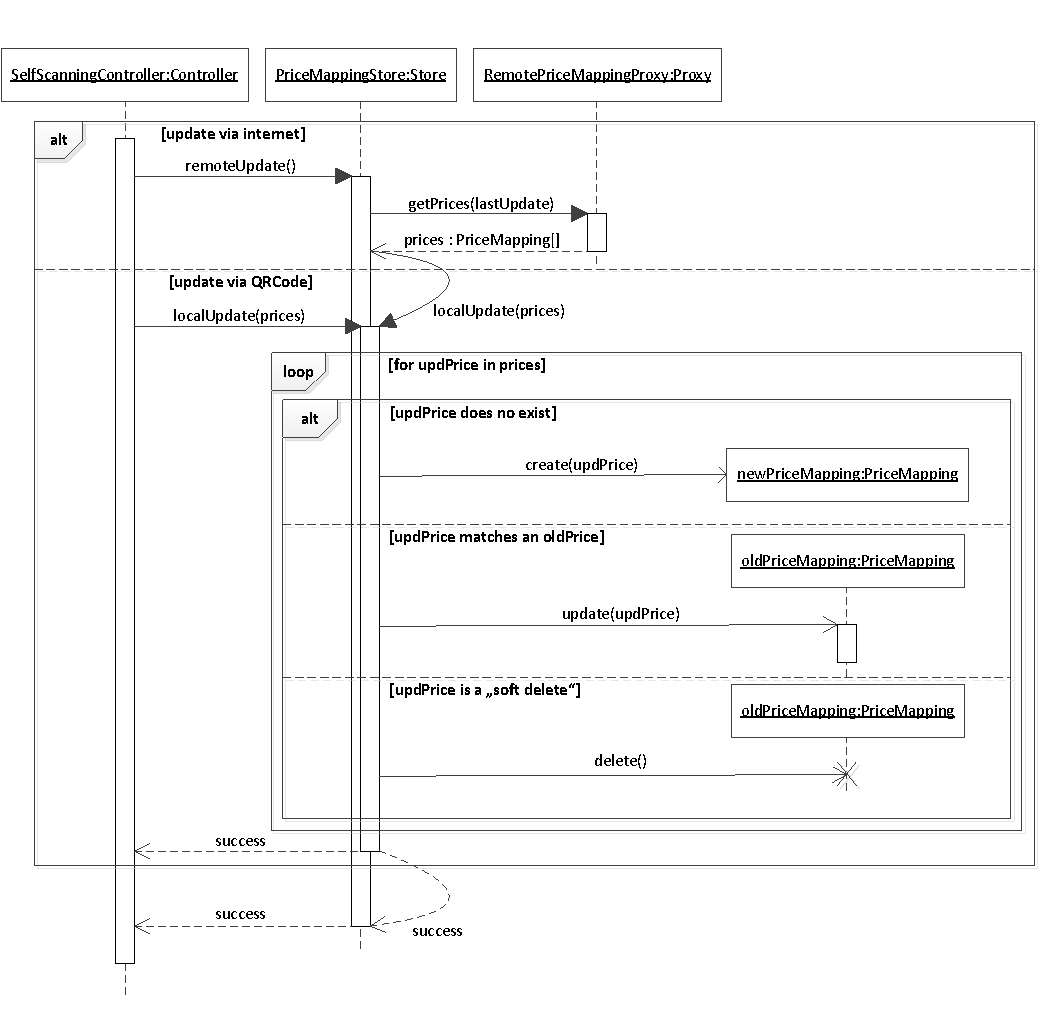
\includegraphics[width=\linewidth]{res/seq_preise-updaten.pdf}
\caption{Der Prozess „Preise updaten“ als Sequenzdiagramm}
\end{figure}

\section{Spezifikation der Schnittstellen}
\subsection{Kasse $\rightarrow$ Smartphone: Einchecken}\label{interface-einchecken}
Um dem Kunden auch dann aktuelle Preisinformationen zu bieten, wenn sein Smartphone nicht mit dem mobilen Internet verbunden ist, werden bei jedem Check-In die lokalen Preisveränderungen (LPVs) der Filiale an das Smartphone übertragen.

Hierfür muss der Kunde vor jedem Einkauf einen QR-Code im Eingangsbereich der Filiale einscannen. Dieser enthält Angaben zu seinem Standort (die Filiale in der er sich aufhält) und alle aktuell gültigen Preisveränderungen dieser Filiale. Die kodierten Informationen lassen sich als konkatenierten String darstellen, dessen einzelnen Bestandteile in der folgenden Tabelle zunächst aufgezählt und anschließend näher erläutert werden.

\begin{table}[H]
  \begin{center}\small\renewcommand{\arraystretch}{1.4}\sffamily % kleinere, serifenlose Schrift & größere Zeilen
  \begin{tabulary}{\textwidth}{ccl}
    Pos. & Länge & Beschreibung\\ \hline
    1 & 3 & Gesellschaftsnummer\\ 
    2 & 3 & Filialnummer\\
    3 & var & Filialpreise\\ 
    4 & 5 & Separator\\ 
    5 & var & Gesellschaftspreise\\
    6 & 5 & Separator\\
    7 & var & Landespreise
   \end{tabulary}      
 \caption{Bestandteile des QR-Codes im Filialeingang}
 \label{tab:uebersicht-vergleich}
 \end{center} 
\end{table}

\begin{seToplist}{1. }
\item[1. ]\textbf{Gesellschaftsnummer} (3 stellig)\label{interface-gnr}\\
	Nummer der Regionalgesellschaft\\
	\textit{Beispiel}: 012 für Gesellschaft 12 (Donaueschingen)
	
\item[2. ]\textbf{Filialnummer} (3 stellig)\\
	Nummer der Filiale\label{interface-fnr}\\
	\textit{Beispiel}: 053 für Filiale 53 (Riedstr. 18 in Lauchringen)
\item[3. ]\textbf{Filialpreise} (variable Länge)\label{interface-fpreise}\\
	Das Filialpreisfeld ist wiederum ein zusammenhängender String aus einzelnen Artikelnummern und Preisen.	Die ersten 5 Stellen enthalten die Artikelnummer (im Falle von kürzeren Artikelnummern werden die Stellen von links mit Nullen aufgefüllt). Die folgenden und auch letzten 5 Stellen enthalten den Preis ohne Dezimaltrennzeichen, wobei die letzten beiden Ziffern als 1/10 und 1/100 Stellen interpretiert werden.
	\begin{seToplist}{Beispiel: }
		\item[\textit{Beispiel}:] 0123400595313379950 für 
		\begin{itemize}
		\item[-] den Artikel 1234 zu einem Preis von 5,95 \euro
		\item[-] den Artikel 31337 zu einem Preis von 99,50 \euro
		\end{itemize}
	\end{seToplist}
	\textit{Wichtige Hinweise}
	\begin{itemize}
	\item[-] Die Artikelnummer 00000 darf nicht vergeben werden! Die Zeichenfolge ist für den Separator (siehe unten) reserviert.
	\item[-] Ein Preis der als 00000 kodiert ist, ist ein sogenannter „soft delete“. D.h. diese Preisveränderung ist nicht länger gültig und muss (falls vorhanden) in der Datenbank des Smartphones entfernt werden. 
	\end{itemize}
	
\item[4. ]\textbf{Separator} (5 stellig)\\
	Das Separatorfeld ist eine reservierte Zeichenkette aus fünf Nullen („00000“). Es dient dazu, die Filialpreise von den Gesellschaftspreisen zu trennen.
	
	\textit{Wichtiger Hinweis}
		\begin{itemize}
		\item[-] Dieses Feld wird nur dann angehängt, wenn Gesellschaftspreise enthalten sind.
		\end{itemize}
		
\item[5. ]\textbf{Gesellschaftspreise} (variable Länge, optional)\\
	Pendant zu den Filialpreisen. Siehe \textit{3. Filialpreise} für weitere Details.
	
\item[6. ]\textbf{Separator} (5 stellig)\\
	Siehe \textit{4. Separator}.
	
	\textit{Wichtiger Hinweis}
			\begin{itemize}
			\item[-] Dieses Feld wird nur dann angehängt, wenn Landespreise enthalten sind.
			\end{itemize}
			
\item[7. ]\textbf{Landespreise} (variable Länge, optional)\\
	Pendant zu Filial- und Gesellschaftspreisen. Siehe \textit{3. Filialpreise} für weitere Details.
\end{seToplist}

Durch den nachfolgenden QR-Code wird ein Beispiel gegeben, das alle oben beschriebenen Informationen enthält. Sein Inhalt kann mit einer gewöhnlichen QRCode-Reader App nachgeprüft werden:

\begin{figure}[H]

\includegraphics[scale=1]{res/qr_eingang}
\caption{Beispielhafter QR-Code mit lokalen Preisveränderungen}
\end{figure}

\texttt{\textcolor{red}{012}\textcolor{orange}{053}\textcolor{blue}{01111}\textcolor{brown}{00000}\textcolor{cyan}{01235}\textcolor{brown}{00050}\textcolor{cyan}{05555}\textcolor{brown}{00000}\textcolor{cyan}{06666}\textcolor{brown}{00000}\textcolor{cyan}{09999}\textcolor{brown}{00000}\textcolor{violet}{00000}\\
\textcolor{cyan}{05555}\textcolor{brown}{00500}\textcolor{cyan}{06666}\textcolor{brown}{00019}\textcolor{cyan}{09999}\textcolor{brown}{00000}\textcolor{violet}{00000}\textcolor{cyan}{01111}\textcolor{brown}{00995}\textcolor{cyan}{01234}\textcolor{brown}{01900}\textcolor{cyan}{01235}\\
\textcolor{brown}{00029}\textcolor{cyan}{05555}\textcolor{brown}{01250}\textcolor{cyan}{06666}\textcolor{brown}{00600}\textcolor{cyan}{09999}\textcolor{brown}{00000}\textcolor{cyan}{12345}\textcolor{brown}{00556}}

\subsection{Smartphone $\rightarrow$ Kasse: Bezahlung}
Nachdem der Kunde alle Waren eingescannt hat, muss der virtuelle Einkaufswagen an das Kassensystem übertragen werden. Hierfür wird auf dem Display des Smartphones ein QR-Code angezeigt, der die Artikelnummern und zugehörigen Mengen aller eingescannten Waren enthält.

Der Inhalt des QR-Codes lässt sich als konkatenierten String darstellen. Seine einzelnen Bestandteile werden im Folgenden näher beschrieben.

\begin{table}[H]
  \begin{center}\small\renewcommand{\arraystretch}{1.4}\sffamily % kleinere, serifenlose Schrift & größere Zeilen
  \begin{tabulary}{\textwidth}{ccl}
    Pos. & Länge & Beschreibung\\ \hline
    1 & 3 & Gesellschaftsnummer\\ 
    2 & 3 & Filialnummer\\
    3 & 3 & Anzahl Artikelpositionen\\ 
    4 & var & Artikeldetails\\ 
    5 & 2 & Anzahl Pfandbons\\
    6 & ? & Pfandbons\\
    7 & 6 & Summe
   \end{tabulary}      
 \caption{Bestandteile des QR-Codes auf dem Smartphone}
 \label{tab:uebersicht-vergleich}
 \end{center} 
\end{table}

\begin{seToplist}{1. }
\item[1. ]\textbf{Gesellschaftsnummer} (3 stellig)\\
	Analog zu \textit{1. Gesellschaftsnummer} in \vref{interface-gnr}.
	
\item[2. ]\textbf{Filialnummer} (3 stellig)\\
	Analog zu \textit{2. Filialnummer} in \vref{interface-fnr}.
	
\item[3. ]\textbf{Anzahl Artikelpositionen} (3 stellig)\\
	Anzahl aller Artikelpositionen (nicht die Gesamtmenge aller Artikel) im Einkaufswagen, zur Berechnung des hierauf folgenden Feldes (Artikelinformationen).
	
		\textit{Wichtiger Hinweis}
			\begin{itemize}
			\item[-] verknüpfte Artikel (z.B. Pfand) sollen hier nicht enthalten sein, da sie auch nicht Bestandteil des nächsten Feldes sind.
			\end{itemize}
	
\item[4. ]\textbf{Artikeldetails} (variabel)\\
	Dieses Feld beinhaltet jeweils die Artikelnummer (5 stellig) mit zugehöriger Menge (2 stellig) jedes eingescannten Produkts. Artikelnr. und Menge werden gegebenenfalls von links mit Nullen aufgefüllt.
	
	\begin{seToplist}{Beispiel: }
			\item[\textit{Beispiel}:] 01234033133701 für 
			\begin{itemize}
			\item[-] 3 Stück von Artikel 1234
			\item[-] 1 Stück von Artikel 31337
			\end{itemize}
		\end{seToplist}
		\textit{Wichtiger Hinweis}
		\begin{itemize}
		\item[-] Verknüpfte Artikel (Pfand) sollen hier nicht enthalten sein. Diese werden von der Kasse erneut dem Kassenbon hinzugefügt.
		\end{itemize}
		
\item[5. ]\textbf{Menge der Pfandbons} (2 stellig)\\
	Menge der im Einkaufswagen enthaltenen Pfandbons. Wird ggf. von links mit Nullen aufgefüllt.
	
\item[6. ]\textbf{Pfandbons} (variabel)\\
	TODO
			
\item[7. ]\textbf{Gesamtsumme} (6 stellig)\\
	An der Kasse zu zahlender Betrag. Die Summe besteht aus 6 Zeichen, ohne Dezimaltrennzeichen. Die letzten beiden Ziffern werden als $\frac{1}{10}$ bzw. $\frac{1}{100}$ Stelle interpretiert. 
\end{seToplist}


\section{Kapitelzusammenfassung}
%TODO Kapitelzusammenfassung schreiben

\chapter{Ergebnisse der Implementierung und Ausblick}
%TODO WRITE !!!


% Anhang der Arbeit
% 
%
\seAppendix{}
\chapter{Anhang}
\section*{Ergänzende Screenshots zu Programm-Listings}
\begin{figure}[H]
	\centering
	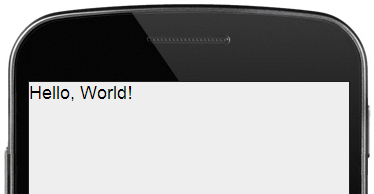
\includegraphics[width=.4\textwidth]{res/hello-world.png}
	\caption[Erste HelloWorld-App]{Erste HelloWorld-App, erzeugt durch \vref{lst:helloworld}\label{abb:helloworld}}
\end{figure}

%
%  Erzeugung eines Glossars
%
% Achtung: Das Glossar wird nur ausgegeben, wenn mindestens ein Eintrag in der Arbeit 
%                definiert wurde
%
%
\newpage
\sePrintGlossary{}


%
% Literaturverzeichnisses
%
%\newpage
\sePrintBibliography{}

%%  Erzeugung von Eintr\"agen im Literaturverzeichnis
%
%  Achtung: in einer Projektarbeit darf da \nocite-Kommando nicht verwendet werden,
%                 da es einen Eintrag im Literaturverzeichnis erzeugt, ohne dass eine 
%                 entsprechende Literaturreferenz im Text der Arbeit angegeben wird
%
%
%



\nocite{DHBW:SG}
\nocite{KM:KS}
\nocite{Dud06}
\nocite{Dud09}
\nocite{Bri:WA}
\nocite{RP:WA}
\nocite{Sch:WAS}
\nocite{BSS:WA}
\nocite{Kor:WA}
\nocite{MK:GWA}
\nocite{ADG:WA}
\nocite{The:WA}
\nocite{BA:WA}
\nocite{Dij:CRT}
\nocite{BC:Cur}
\nocite{Par:ECP}
\nocite{Bro:SBE}
\nocite{GI:ADI}
\nocite{GI:AZI}
\nocite{Den:CD}
\nocite{LMS:Icb}
\nocite{Fre:SIF}




%
% Festlegung des grundlegenden Formatierungsstils des Literaturverzeichnis
%
\bibliographystyle{jurabib}

% Eigentliche Ausgabe der in der Arbeit verwendeten Quellen
%
%
% Angabe der bib-Dateien, in denen die Quellen beschrieben sind;
% die Angabe geht davon aus, dass eine wa.bib-Datei in demselben 
% Verzeichnis liegt, wie se-ba-vorlage.tex
%

% 2012-02-06
%
% Umbenennung von Literatur- in Quellenverzeichnis
% 
%\renewcommand*{\bibname}{Quellenverzeichnis}
\seBibliography{wa}


%
% Erzeugung der ehrenw\"ortlichen Erkl\"arung
%
% Der optionale Parameter kann verwendet werden, um f\"ur das Thema der Arbeit eine 
% andere Formatierung vorzunehmen; das sollte in der Regel nicht erforderlich sein;
% ausserdem besteht die Gefahr inkonsistenter Titel auf dem Titelblatt und in der 
% ehrenw\"ortlichen Erkl\"arung
%
%\seEhrenwoertlicheErklaerung{} % dieses Kommando sollte standardm\"assig verwendet werden
\seEhrenwoertlicheErklaerung[\seThemaWaArbeit{}]


\end{document}